%----------------------------------------
% Preamble to set up the document
%----------------------------------------
\documentclass{article}

% set up packages (you shouldn't need to touch this)
\usepackage{graphicx}  % required to insert images
\usepackage{hyperref}  % for hyperlinks
\usepackage[svgnames]{xcolor}  % to change hyperlink colors
\colorlet{linkcolour}{DarkBlue}
\hypersetup{colorlinks=true, linkcolor=linkcolour, citecolor=linkcolour, urlcolor=linkcolour,}

% Margins
\topmargin=-0.45in
\evensidemargin=0in
\oddsidemargin=0in
\textwidth=6.5in
\textheight=9.0in
\headsep=0.25in

% use a sans serif font
\renewcommand{\familydefault}{\sfdefault}

%----------------------------------------
% Step 1: Edit the lecture title
%----------------------------------------
\title{
Lecture 11: Causation and Experiments \\  % Lecture title
Modeling Social Data, Spring 2017 \\   % Course title
Columbia University                    % School
}

%----------------------------------------
% Step 2: Edit your name and the date
%----------------------------------------
\author{Robbie Netzorg}                     % Scribe's name
\date{April 20, 2017}                % Lecture date

\begin{document}

\maketitle


%----------------------------------------
% Step 3:
% Rename uni.tex to match your uni,
% edit the filename accordingly below,
% and put your notes in this file
%----------------------------------------
%----------------------------------------
% Write your notes here
%----------------------------------------

\section{Prediction vs. Causation}
So far, we've been trying to understand data to make a forecast. Causation, however, is to try and anticipate what will happen. For example, people out on the street holding umbrellas might predict rain, but it does not cause rain. \\
\subsection{Types of Causal Inference}
Not all types of causal inference are created equal. For example, asking ``What makes Apple so successful?'' brings with it different challenges than the question ``What effects does hospitalization have on health?''\\\\
\textbf{Reverse Causal Inference}: Looking at the Causes of Effects. Generally quite hard to do, nearly impossible. There are tendencies to have tons of effects, making it difficult to isolate out causes. The Apple question is an example of Reverse Causal Inference. \\ \\
\textbf{Forward Causal Inference}: Looking at the Effects of Causes. While it's still difficult to do properly, it's less contentious and can lead to actual conclusions. Most science relies on Forward Causal Inference to connect causes to their effects because properly conducted experiments can isolate out the causal effects in data. The hospitalization question is an example of this.\\

\subsection{The Problem with Forward Causal Inference}
Great! Now that we have our method, we should be able to grab any old dataset and do some Forward Caussal Inference magic and we're good to go! Well, not exactly. If we use an arbitrarily gathered dataset, that dataset can inherently contain biases that distort out the causal effects we hope to study. These are known as \textit{confounds}. For example, returning to the hospitalizaion example, health of an individual determines whether or not they end up going to the hospital. In the extreme case, where all sick people go to the hospital and all healthy people stay home, we would find that hopitalization reduces your hance of survival! The problem here is that we can't observe the effect of sick people not going to the hopsital. \\
The above example gets into the issue of \textbf{selection bias}. In any kind of data, there's a selection bias present, whereby the group of people has been pre-selected, causing problems with trying to isolate causal relationships. In all situations, the observed difference between two groups can be described by the following formula:

\begin{equation}
  \Delta_{obs} = causal\ effect - selection\ bias
\end{equation}

Selection bias is usually negative.

\subsection{Simpson's Paradox}
Selection bias can be so large that observational and causal estimates give opposite effects. In other words, you can get completely flipped answers by not conditioning on the right variables. For example, when comparing two algorithms, you can find that one algorithm apparently outperforms the other, but, in reality, the opposite is true:
\begin{figure}[ht]
  \begin{center}
    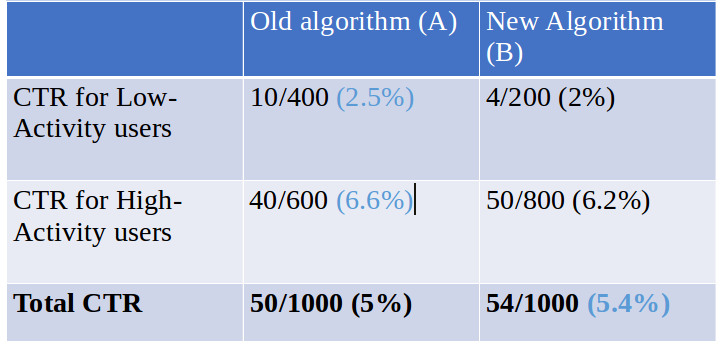
\includegraphics[width=0.5\textwidth]{figures/fig1.png}
    \caption{ Simpson's Paradox in action }
    \label{fig:fig1}
  \end{center}
\end{figure}
Now what? Simpson's Paradox seems to suggest that, if we're not careful, we're going to be sent down endless rabbit holes, never knowing when exactly we've reached the conclusion of our analysis. Fear not! Science has an answer!

\section{Experiments}
\subsection{The Light at the End of the Tunnel}
\textbf{Counterfactuals}: To isolate the causal effect in the data, we have to change one things and one thing only. We try to clone the current universe and just change one thing in the new universe. This allows us to compare reality to the counterfactual. Where reality is what happened, whereas the counterfactual is what would've happened.  \\ \\
To accomplish this feat, we introduce a sense of randomness into the world. We randomly assign individuals to World A and World B where the only difference between the two is the one change we've made. In this matter, we've reframed the previous formula:

\begin{equation}
  \Delta_{obs} = causal\ effect 
\end{equation}

Selection bias has, for the most part, been removed due to the introduction of randomization. With this technique, then, we have constructed a means of measuring causal effects.

\subsection{The Trade-Off: Internal Validity vs. External Validity}
Although we managed to generate a means of measuring causation in datasets, the fact of the matter is that everything isn't perfect. Randomization is easy to write about but difficult to accomplish in practice, running into ethical or feasibility concerns. Experiments often are costly and take time to set up. Finally, it is often \textit{painstakingly difficult} to create convincing parallel worlds. Due to this issues, scientists make trade-offs when constructing experiments. \\ \\

\textbf{Internal Validity}: Ensuring that the observed changes are the result of the change of the world and that change early. The question becomes: Could anything other than the treatment (aka the change) produce this outcome? Lab Experiments are great at controlling for Internal Validity. Experimenters have great control over introducing changes in the population. Trying to measure internval validity outside of a lab environment is difficult, however, since the real world introduces many different variables that could influence the result. \\ \\

\textbf{External Validity}: Ensuring that the observed changes are not just observable in the experiment but hold in other settings as well. For example, would the tested medication be effective outside of a clinical trial? Field experiments that take place outside of a lab environment are great for external validity. They generalize better and apply to real-world situations. Lab experiments, on the other hand, run into problems with generalzation, since tested populations are homogeneous (see W.E.I.R.D.) and the environment is artifical.

\subsection{The Promise of the Internet}
Research has historically been bounded by the previous trade-off, but the introduction of the Internet has the potential to rework this system entirely. Properly conduted Internet experiments have hte potential to weave together the benefits of the lab and the field, allowing researchers to turn the historical trade-off into more of a spectrum. The hope is that, one day, researchers will develop a system that allow the mass-testing of various behavioral experiments online.

\section{Natural Experiments}
\subsection{When Reseachers get Lucky}
Sometimes, nature does the experimenter's job for them. Some systems have introduced features of experiments that effectively isolate causal effects. Although this is a rare occurence, it is useful to keep an eye out for and allows for otherwise difficult questions to be answered. \\ \\
\textbf{As-if Random}: Sometimes people are randomly distributed already without the intervention of the experimenter. The best example of this is John Snow's study of the cholera outbreak in London. Because he found that people were exposed to water sources as-if randomly, he was able to demonstrate that there was a causal link between contaminated water and sickness. The goal for this type of study is to find the features in nature that are random in themselves. \\ \\
\textbf{Instrumntal Variables}: Sometimes human systems randomly assign human beings to different fates. In otherwords, an instrument independently shifts the distribution of the treatment. An example of this is the draft lottery, whereby people were randomly assigned to military service or not. With this situation, it is possible to ask what the effects of military service are on an individual's life. This situation doesn't necesarily have complete randomness, but the system has \textit{some randomness} that allows you, as a researcher, to infer out the causal relationship.
\begin{figure}[ht]
  \begin{center}
    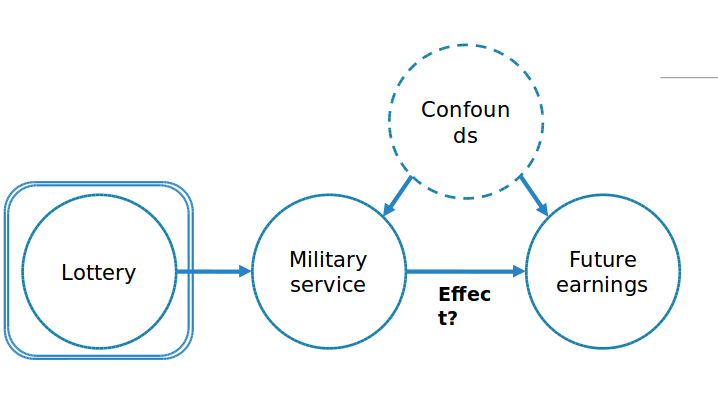
\includegraphics[width=0.5\textwidth]{figures/fig2.png}
    \caption{ Example of Instrumental Variable in Military Lottery }
    \label{fig:fig2}
  \end{center}
\end{figure}

\end{document}

%%% Local Variables:
%%% mode: latex
%%% TeX-master: t
%%% End:
